\documentclass[article,colorback,accentcolor=tud4c]{tudreport}
\usepackage[english]{babel}

\usepackage[stable]{footmisc}
\usepackage{hyperref}
\usepackage{color}

\usepackage{longtable}
\usepackage{multirow}
\usepackage{booktabs}

\usepackage{enumitem}
\setenumerate[1]{itemsep=0pt,partopsep=0pt,parsep=\parskip,topsep=5pt}
\setitemize[1]{itemsep=0pt,partopsep=0pt,parsep=\parskip,topsep=5pt}
\setdescription{itemsep=0pt,partopsep=0pt,parsep=\parskip,topsep=5pt}

\renewcommand {\thetable} {\arabic{section}.\arabic{table}}
\renewcommand {\thefigure} {\arabic{section}.\arabic{figure}}

\hypersetup{%
  pdftitle={TUD Corporate-Design f"ur {\LaTeX}},
  pdfauthor={C. v. Loewenich und J. Werner},
  pdfsubject={Beispieltext},
  pdfview=FitH,
  pdfstartview=FitV
}

\setcounter{seclinedepth}{1}

%%% Zum Tester der Marginalien %%%
  \newif\ifTUDmargin\TUDmarginfalse
  %%% Wird der Folgende Zeile einkommentiert,
  %%% werden Marginalien gesetzt.
  % \TUDmargintrue
  \ifTUDmargin\makeatletter
    \TUD@setmarginpar{2}
  \makeatother\fi
%%% ENDE: Zum Tester der Marginalien %%%

\newlength{\longtablewidth}
\setlength{\longtablewidth}{0.7\linewidth}
\addtolength{\longtablewidth}{-\marginparsep}
\addtolength{\longtablewidth}{-\marginparwidth}


% \settitlepicture{tudreport-pic}
% \printpicturesize

\title{Industrial Internship Report}
\subtitle{Letian Feng}
\subsubtitle{2255840\\
ETiT - Datentechnik\\
letian.feng@hotmail.com\\
31.12.2017
}
\setinstitutionlogo[width]{SAP_logo}

\begin{document}
\maketitle
\begin{abstract}

This report records my experience as a software developer intern in the team \textit{Big Data Vora} of the company SAP headquarters in Walldorf, Baden-W{\"u}rttemberg, Germany.

SAP(\textbf{S}ystems, \textbf{A}pplications \& \textbf{P}roducts in Data Processing), is the world leader in enterprise applications in terms of software and software-related service revenue. 
The team \textit{Big Data Vora} focuses on processing big data in distributed systems, especially on computing clouds like Amazon AWS and Microsoft Azure. 
Now this team is working on \href{https://www.sap.com/products/data-hub.html}{\textcolor{blue}{SAP Data Hub}}, which is a brand new data processing platform and the base of SAP's next generation products like Leonardo. 
In the end, SAP Data Hub should be able to run both SAP and non-SAP services, just like SAP's motto - Run Simple.

From my view as a developer, SAP Data Hub consists of 3 parts: 
\begin{itemize}\itemsep-\the\parsep
	\item SAP Vora, infrastructure, distributed database system for big data processing. It contains a series of data processing engines, a transaction coordinator, and several interfaces to import data from different sources;
 	\item vFlow, backend service. It is a pipeline system helping customers to define their data flows running on SAP Vora or other data processing tools;
 	\item Web UI, frontend interface for the vFlow.
\end{itemize}

More detailed information about SAP Data Hub will be given in the following sections.

My work is almost all about an operator in the vFlow system - \textbf{Livy Spark Submit}. It submits data processing jobs to a Livy server in the remote cluster, then it retrieves the execution results or error information when the jobs succeed or fail.

In the past, only users on an internal node could submit data processing jobs to the cluster, external users have to remotely login as an administrator and then submit their jobs, so it is very inefficient and could be every insecure. With the Livy operator, external users could submit their jobs remotely to any cluster containing a Livy server, but only authenticated users' jobs could be accepted. This operator provides users the opportunity to scale out their computing capacity transparently, e.g. deploy more cluster; on the other hand, it gives cluster administrators the ability to protect their computing nodes from unauthenticated users. In short, the Livy operator kills two birds with one stone.

Basically, my contribution could be split into 4 parts: 

\begin{itemize}\itemsep-\the\parsep
	\item Proof of concept;
	\item Source code implementation;
	\item Unit tests \& docker based integration tests;
	\item Error handling/monitoring improvement.
\end{itemize}

To accomplish the above tasks, following technologies and programming languages were used: 

\begin{itemize}\itemsep-\the\parsep
	\item 
	\href{http://hadoop.apache.org/}{\textcolor{blue}{Hadoop}}, \href{https://spark.apache.org/}{\textcolor{blue}{Spark}},
	\href{https://en.wikipedia.org/wiki/Linux}{\textcolor{blue}{Linux}}, \href{https://www.docker.com}{\textcolor{blue}{Docker}}, \href{https://livy.incubator.apache.org/}{\textcolor{blue}{Livy}}, \href{https://www.sap.com/products/hana-vora-hadoop.html}{\textcolor{blue}{SAP Vora}}, \href{https://web.mit.edu/kerberos/}{\textcolor{blue}{Kerberos}}, \href{https://git-scm.com/}{\textcolor{blue}{Git}}, \href{https://en.wikipedia.org/wiki/Markdown#Implementations}{\textcolor{blue}{Markdown}},
	\href{https://www.wireshark.org/}{\textcolor{blue}{Wireshark}} \& \href{https://kubernetes.io/}{\textcolor{blue}{Kubernetes}};
	\item 
	\href{https://golang.org/}{\textcolor{blue}{Go}}, \href{https://www.gnu.org/software/bash/}{\textcolor{blue}{Bash}} \& \href{https://www.scala-lang.org/}{\textcolor{blue}{Scala}}. 
\end{itemize}

The report introduces a lot of technical details, encountered challenges and even some bugs. Features will be illustrated by pictures, but no source code will be shown due to confidential reasons. All code were pushed into SAP's internal GitHub.
\end{abstract} 
\newpage

\tableofcontents
%\part{Lorem Ipsum (\textbackslash part)\label{part_lorem}}
\newpage

\section{Introduction}
\setcounter{table}{0}
\setcounter{figure}{0}

SAP Data Hub is a DataOps management solution that enables agile data operations across the enterprise. It supports data sharing, pipelining, and governance of all data in the connected landscape.

The SAP Data Hub product is composed of several components:
\begin{itemize}\itemsep-\the\parsep
\item An application tier (control plane) based on SAP HANA extended application services (XS), advanced model.
\item The core distributed runtime (based on SAP Vora) installed on a Kubernetes cluster.
\item Extensions to the Spark environment on a Hadoop cluster.
\item The SAP Data Hub adapter agent installed on one edge node of the Hadoop environment.
\end{itemize}

Figure 1.1 outlines the deployment view of SAP Data Hub.

\begin{figure}[!h]
   	\centering
   	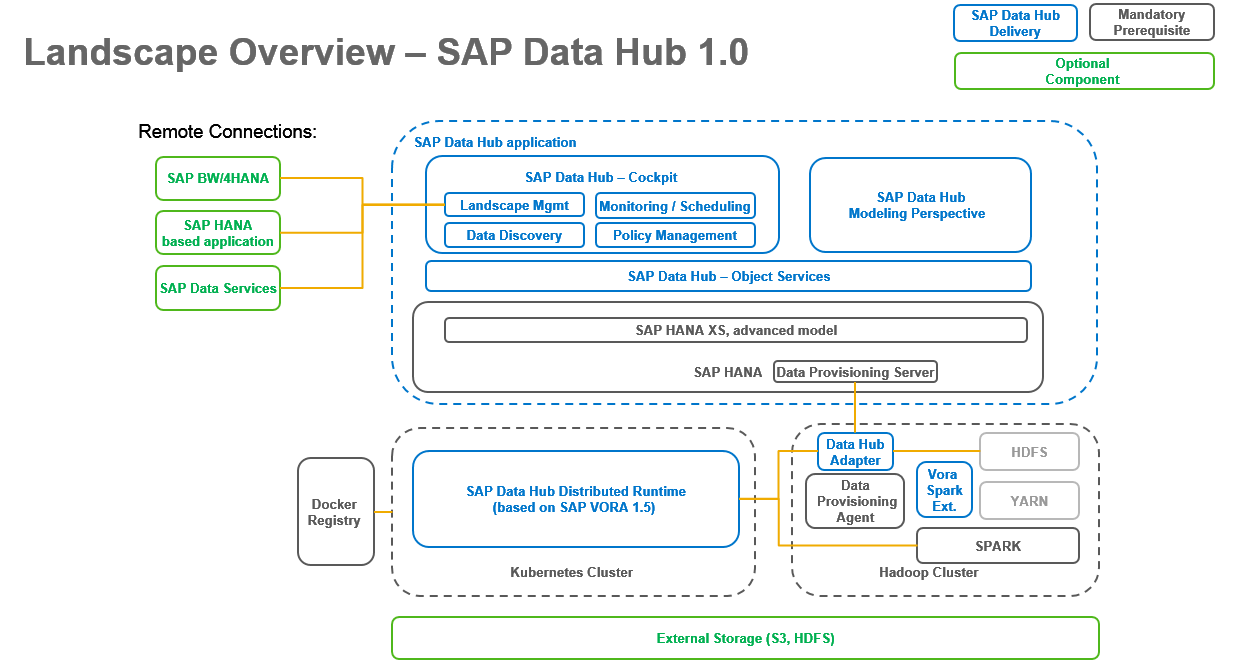
\includegraphics[width=\textwidth]{architecture}
   	\caption{Architecture of SAP Data Hub}
\end{figure}

All data services are running in the top level - the application tier. With Data Hub Cockpit, data services can generate data processing pipelines, each pipeline contains a series of operations, e.g. load data from a file in HDFS, filter something, and then output in the web page. Sometimes users want to DIY their own data processing pipelines, then they can use Data Hub Modeling Perspective, which is actually the web UI of vFlow mentioned in the abstract. Pipelines will be passed from Data Provisioning Server to Data Hub Adapter. 

Data Hub Adapter is the central communication endpoint for operations performed from SAP Data Hub application on SAP Data Hub Distributed Runtime(SAP Vora, vFlow, and Hadoop). With help of Data Hub Adapter, pipelines will be sent to the Distributed Runtime and be executed there.

\begin{figure}[!h]
	\centering
	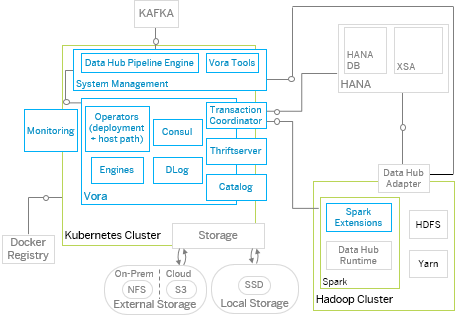
\includegraphics{vora}
	\caption{A high-level overview of the SAP Data Hub Distributed Runtime}
\end{figure}

As shown in the figure 1.2, we can know more about SAP Data Hub Distributed Runtime and how a pipeline is executed. First, the Data Hub Adapter gives the pipeline received from the application tier to Data Hub Pipeline Engine in the Kubernetes cluster. If the pipeline contains a Spark/Vora job, this job will be sent back to Data Hub Adapter, then a Spark client will submit the job to the scheduler YARN. YARN will allocate computing resources for it. If it's only a simple Spark job, it runs only in the Hadoop cluster; but if it's also a Vora job, an external library "Vora Spark Extension" will be invoked to submit queries to Vora Transaction Coordinator(TC) in the Kubernetes cluster. TC controls the execution of queries on several engines for different functions - relational, graph, time series and document engine. After all queries are executed, results will be returned, Spark jobs and the pipeline will be finished step by step, final results will be displayed on the web UI. 

However, in this report, we don't need to discuss all details of SAP Data Hub. Figure 1.3, which only shows the interfaces of SAP Data Hub, is a easier way to understand it:

\begin{figure}[!h]
	\centering
	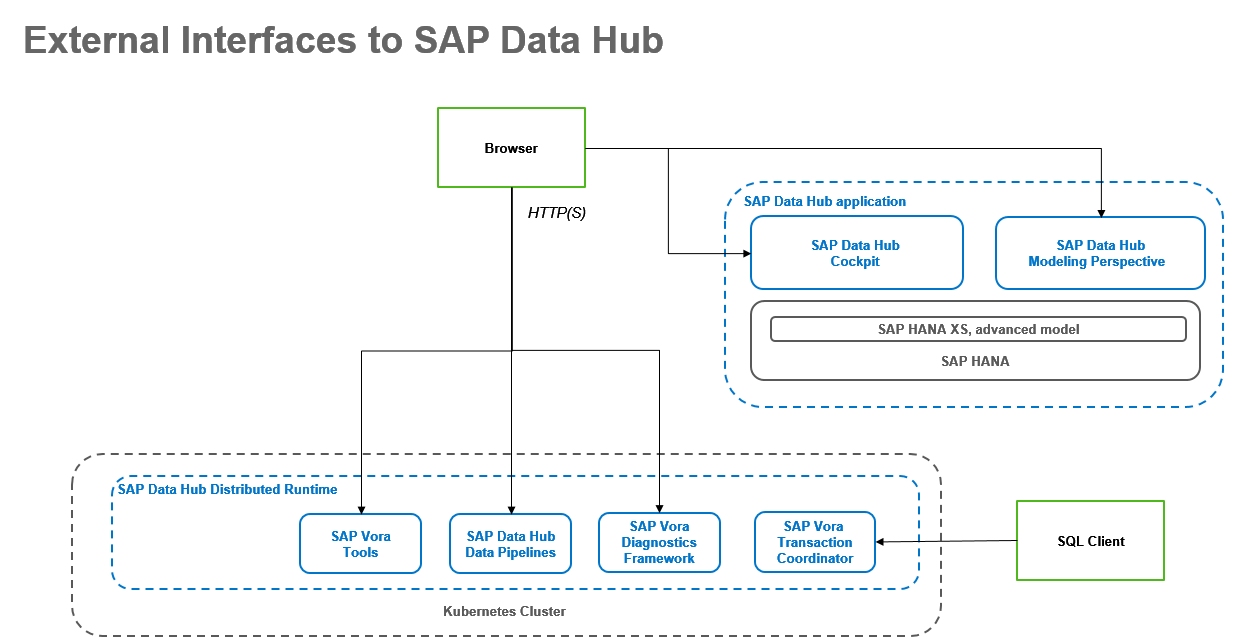
\includegraphics[width=\textwidth]{interfaces}
	\caption{Interfaces of SAP Data Hub}
\end{figure}

Users always use their web page browser to access SAP Data Hub. They use either a data service in SAP Data Hub Cockpit to generate a data processing pipeline, or use SAP Data Hub Modeling Perspective to DIY a pipeline. The pipeline will be given to a SQL client, and this SQL client will communicate with the Transaction Coordinator in SAP Data Hub Distributed Runtime, so that data could be processed correctly. During the execution users should also be able to monitor pipeline's status via Diagnose Framework, and they can check the final results with Vora Tools after the pipeline is finished. Both Diagnose Framework and Vora Tools are accessible in the browser.

\newpage

\section{Proof of Concept}
\setcounter{table}{0}
\setcounter{figure}{0}

SAP Data Hub version 1.0 was released in September 2017, and then version 1.2 was released in December 2017. As the core component of the Data Hub Distributed Runtime, SAP Vora also keeps evolving itself. When I started my internship, Vora released v1.4, then in September Vora v2.0 was released, and in December was Vora v2.1. Their architectures are shown in the following pictures:

In Vora v1.4, there were many components, their relationships and dependencies were very complex, both Vora engines and Spark nodes are running on the same cluster.

\begin{figure}[!h]
	\centering
	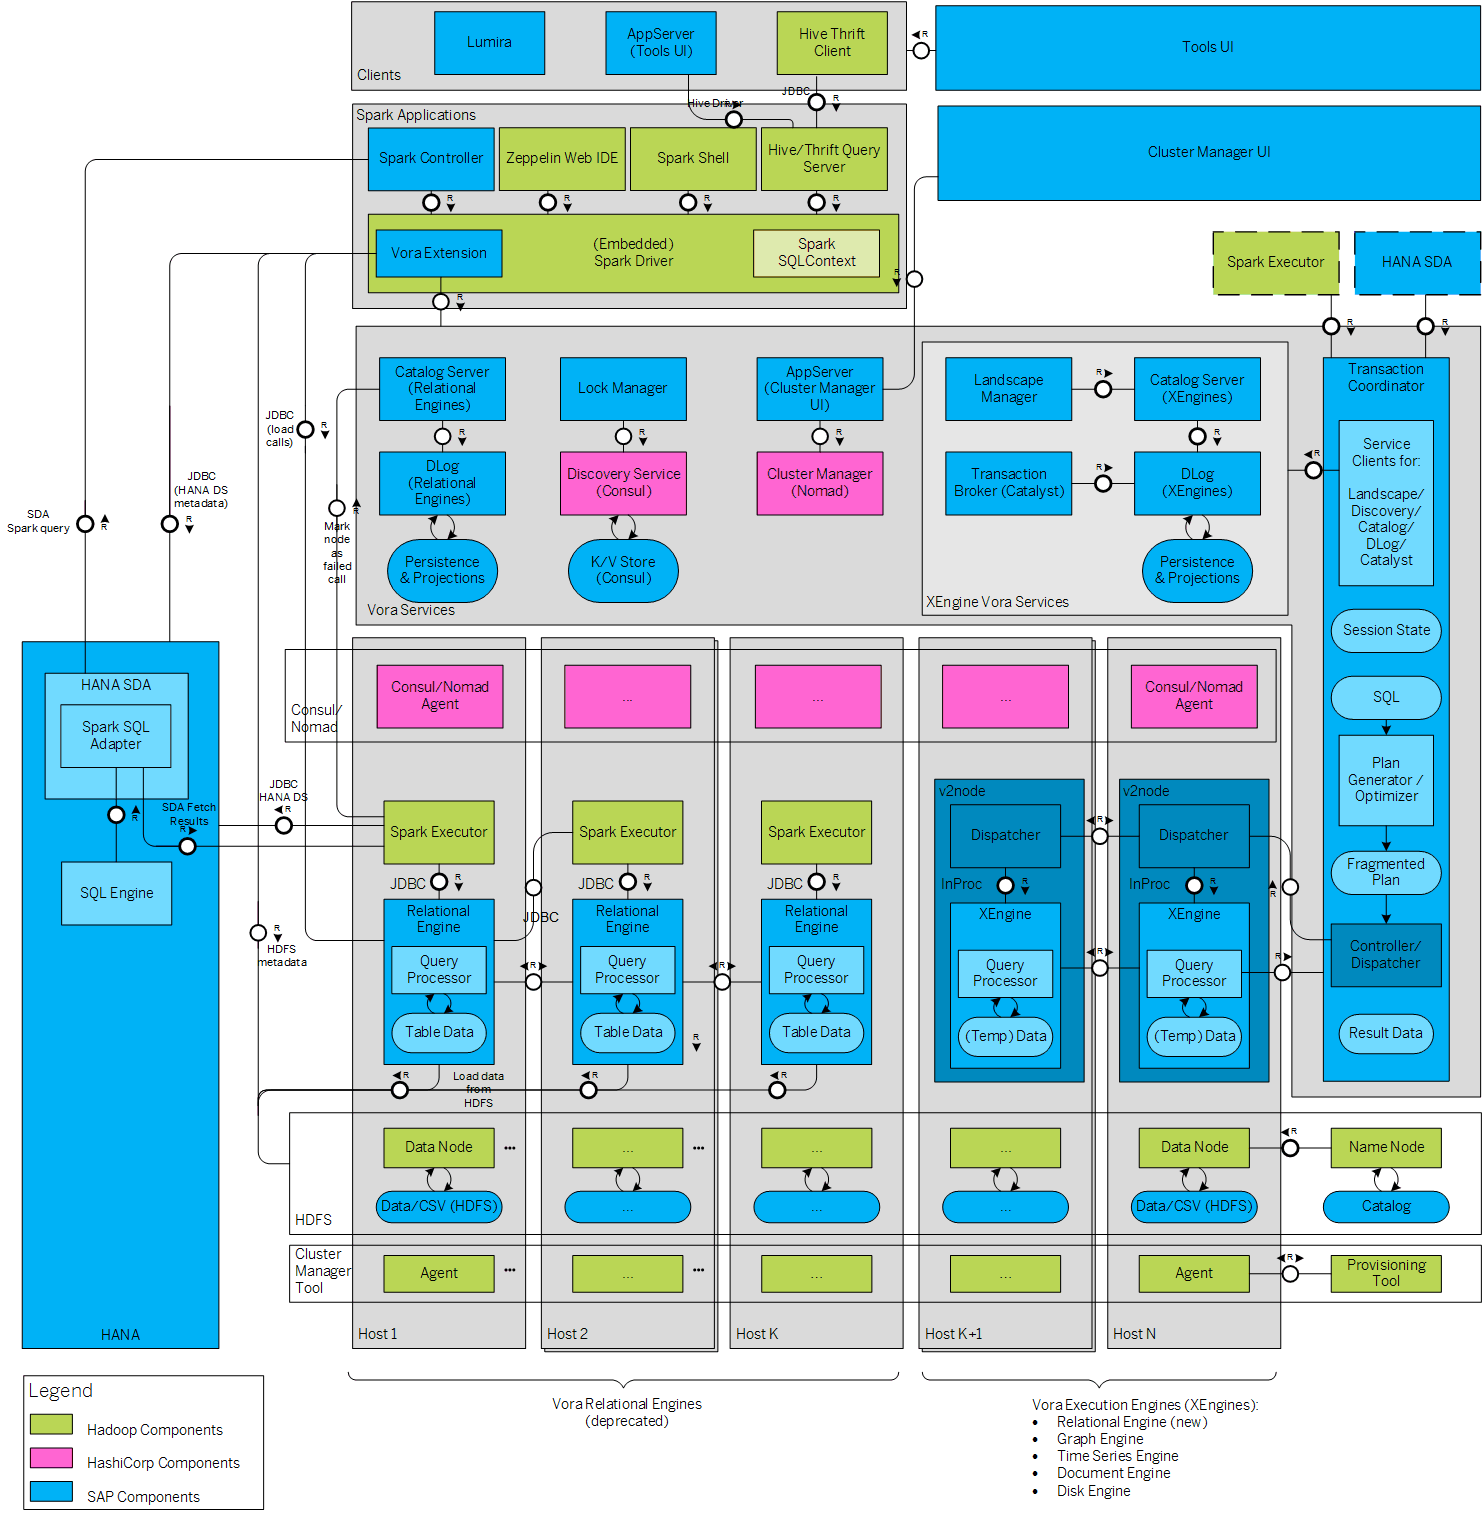
\includegraphics[width=0.9\textwidth]{vora14}
	\caption{SAP Vora Architecture version 1.4}
\end{figure}

In Vora v2.0, all Vora components were encapsulated in Docker\footnote{Docker is a tool that can package an application and its dependencies in a virtual container that can run on any Linux server. This helps enable flexibility and portability on where the application can run, whether on premises, public cloud, private cloud, bare metal, etc.} containers and managed by a Kubernetes\footnote{Kubernetes is an open-source platform designed to automate deploying, scaling, and operating application containers. It supports a range of container tools, including Docker.} cluster, only few things like Spark workers and the Vora Spark Extension remain in the original Hadoop cluster. In this way, all Vora services are separated from the computing resources in the Hadoop cluster. With help of Kubernetes, all Vora services could be easily deployed and seamlessly updated or reverted.

\begin{figure}[!h]
	\centering
	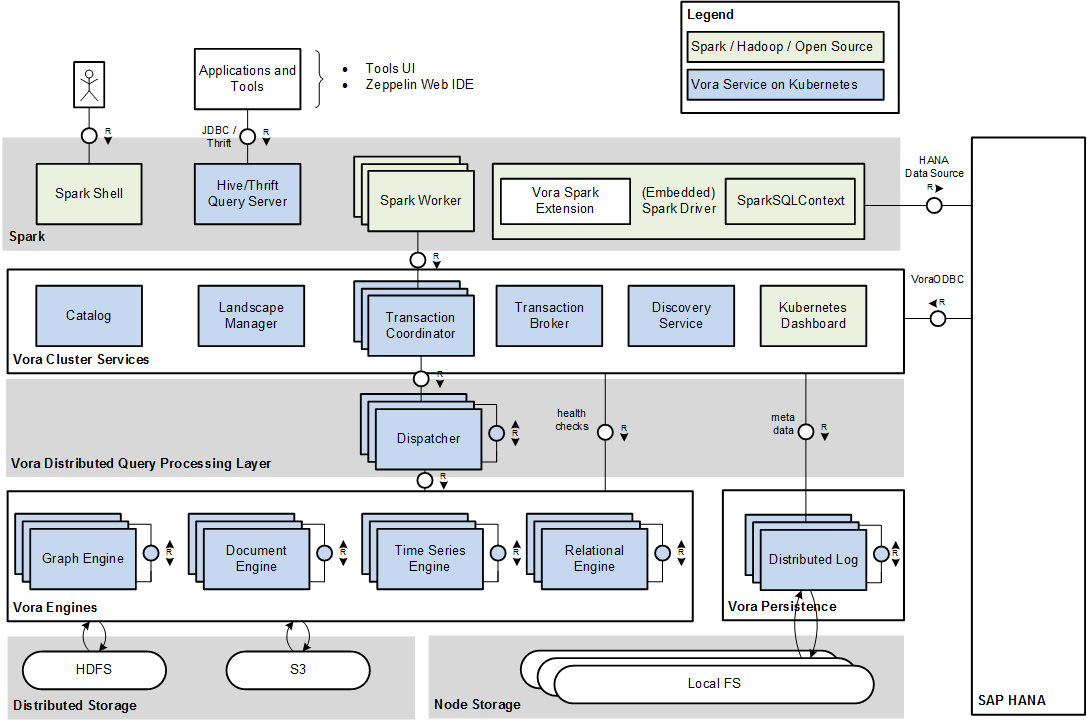
\includegraphics[width=0.9\textwidth]{vora20}
	\caption{SAP Vora Architecture version 2.0}
\end{figure}

Finally, in Vora v2.1, Livy shows up for the first time, and it becomes the most preferred Spark client in the Hadoop cluster to submit Spark/Vora jobs.

\begin{figure}[!h]
	\centering
	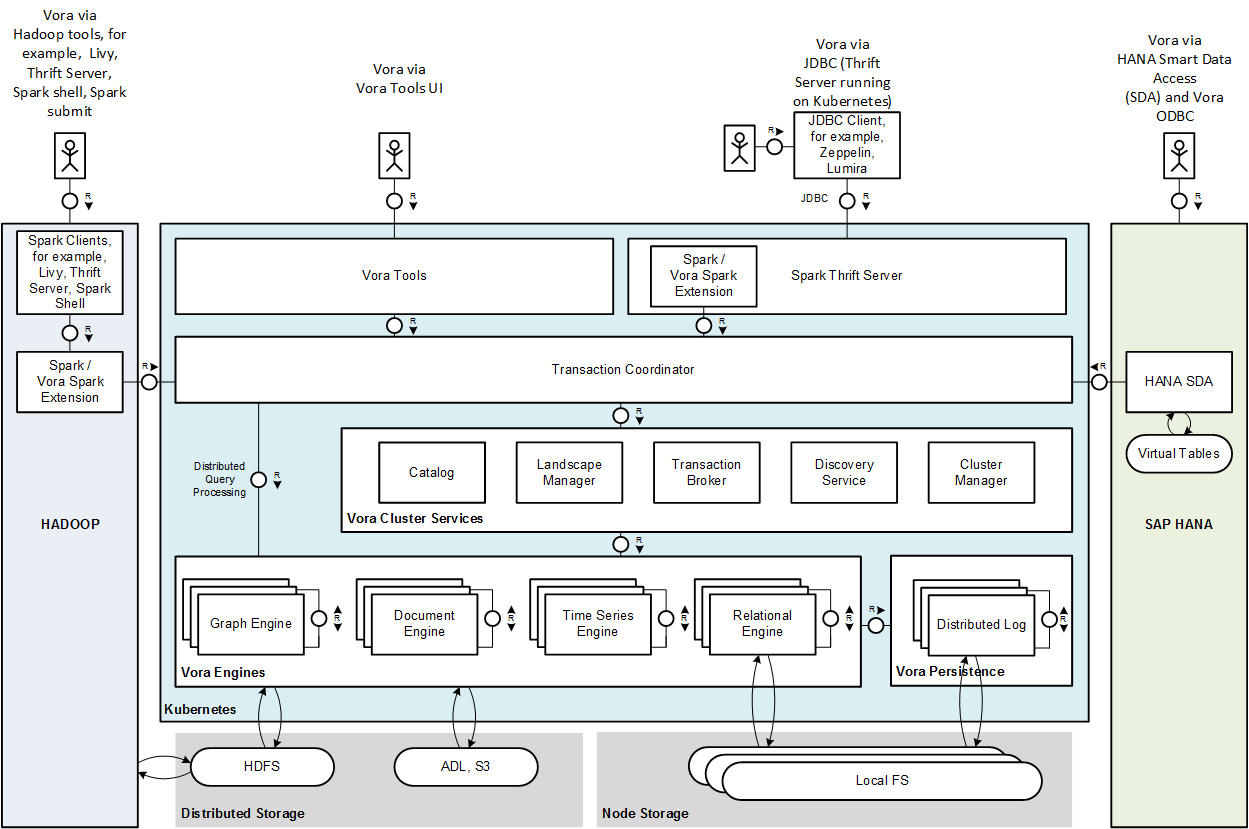
\includegraphics[width=0.9\textwidth]{vora21}
	\caption{SAP Vora Architecture version 2.1}
\end{figure}

The 2 changes in v2.0 and v2.1 have very important effects:

\begin{enumerate}
	\item Separate Vora from the Hadoop cluster, put it in a Kubernetes cluster:
	\begin{itemize}
		\item Lower system coupling, higher computing efficiency;
		\item Easier to manage and secure Vora components;
		\item Kubernetes makes it possible to update or revert Vora version seamlessly.
	\end{itemize}
	\item Add a Spark client Livy in the Hadoop cluster:
	\begin{itemize}
		\item Possible to submit jobs to a remote Hadoop cluster;
		\item Possible to submit jobs with username, only authenticated users' requests could be passed, higher security;
		\item A Vora cluster could access multiple Hadoop clusters,scale out computing resources, not scale up.
	\end{itemize}
\end{enumerate}

Since those 2 changes mean a lot, they must be proved before being implemented - Proof of Concept, as known as POC. I was responsible to  the POC of Livy, it consists of 4 steps, I will describe them in the following 4 subsections.

	\subsection{Prove that Livy could submit Spark jobs to a simple cluster}
	Actually, submission of Spark jobs is exactly Livy's function\footnote{Livy's official definition: \textit{Apache Livy is a service that enables easy interaction with a Spark cluster over a REST interface. \textbf{It enables easy submission of Spark jobs or snippets of Spark code}, synchronous or asynchronous result retrieval, as well as Spark Context management, all via a simple REST interface or an RPC client library.}}. However, a software engineer should never simply believe in documentations, there are usually hundreds of bugs in every software. Therefore, experiments are always required before a technology is used in the production environment.
	
	Before we start to prove, let me explain what is a Spark job and how it is submitted in the traditional way. A job is actually an application that running on a cluster. Once an user application is bundled, it can be launched using the spark-submit\footnote{The spark-submit script in Spark's bin directory is used to launch applications on a cluster. It can use all of Spark’s supported cluster managers through a uniform interface.} script. This script takes care of setting up the classpath with Spark and its dependencies, and can support different cluster managers and deploy modes that Spark supports. The format of executing spark-submit is:
	
	\noindent\textbf{spark-submit --class <main-class> --master <master-url> ... <application-jar> [application-arguments]}
	
	Obviously, to submit a job, we need at least a class name, a path to the application JAR\footnote{A JAR (Java ARchive) is a package file format typically used to aggregate many Java class files and associated metadata and resources (text, images, etc.) into one file for distribution.}, a cluster manager. For example, the following command runs a Pi-calculating-job saved in the default Spark examples JAR on a cluster managed by YARN\footnote{Hadoop YARN, a platform responsible for managing computing resources in clusters and using them for scheduling users' applications.}, the JAR file is stored in HDFS\footnote{Hadoop Distributed File System(HDFS), a distributed file-system that stores data on commodity machines, providing very high aggregate bandwidth across the cluster.} and this job will be split into 10 partitions:
	
	\noindent\textbf{spark-submit --class org.apache.spark.examples.SparkPi   --master yarn-cluster hdfs:///tmp/spark-examples.jar 10}
		
	Now let's see how can we submit a Spark job through Livy. First, we need to install Livy on our cluster and run Livy's RESTful service\footnote{Representational state transfer (REST) or RESTful web services are a way of providing interoperability between computer systems on the Internet. REST-compliant Web services allow requesting systems to access and manipulate textual representations of Web resources using a uniform and predefined set of stateless operations.}. According to \href{https://livy.incubator.apache.org/docs/latest/rest-api.html}{\textcolor{blue}{Livy's REST API}}, we can send POST/GET/DELETE requests to the Livy server to submit, monitor, and cancel Spark jobs. To submit a job, we need to send a POST request with data options like "file", "className", and "args" to the URI(Uniform Resource Identifier) /batches. 
	
	In command line mode, we usually use the tool curl\footnote{cURL is a computer software project providing a library and command-line tool for transferring data using various protocols.} to send requests, for example, the following command sends a job submission request which is identical as the spark-submit request above:
	
	\noindent\textbf{curl -v \$LIVY\_URL/batches -X POST -H "Content-Type:application/json" --data '\{"file":"/tmp/spark-examples.jar", "className":"org.apache.spark.examples.SparkPi", "args":["10"]\}'}
	
	After sending this POST request to Livy and checking the cluster manager YARN's UI, we could find that a job "org.apache.spark.examples.SparkPi" is accepted and finished with a result like "Pi is roughly 3.13918". So it is proved that Livy could submit Spark jobs to a simple cluster.
		
	\subsection{Prove that Livy could submit Vora jobs to a simple cluster}
	
	First of all, I deployed a Vora cluster without Kerberos and installed Livy, then started services HDFS, YARN, Livy, and Vora Tools. After uploaded the Vora Spark Extension "spark-sap-datasources.jar" to the HDFS, I sent the Vora job submission request to Livy:
	
	\noindent\textbf{curl -v \$LIVY\_URL/batches -X POST -H "Content-Type:application/json" -H "X-Requested-By: hdfs" --data '\{"file": "/tmp/spark-sap-datasources.jar", "className":"com.sap.spark.vora.examples.LoadDataIntoVora","args":["10"]\}'}
	
	Because the Vora cluster enables the CSRF protection\footnote{\textbf{Cross-site request forgery is a type of malicious exploit of a website where unauthorized commands are transmitted from a user that the web application trusts.}} by default, this request has an additional header "X-Requested-By: hdfs". The application jar is not spark-examples.jar any more, but our Vora Spark Extension. This job does nothing but load data from some csv-files saved in HDFS to Vora. As same as in the subsection 2.1, this job could always be accepted and executed by YARN. If we check the Vora Tools we started at the beginning, we can find that data is already loaded into Vora. So it is proved that Livy could submit Vora jobs to a simple cluster.
		
	\subsection{Prove that Livy could submit Spark jobs to a Kerberized cluster}
	
	In the last 2 subsections, we have proved that Livy fulfills our expectation for remote submission. However, Livy has a feature - impersonation. It provides users the possibility to submit jobs as other users and even administrator, this could lead to security problem, so Kerberos is introduced to secure the Vora cluster.
	
	Kerberos is a computer network authentication protocol that works on the basis of tickets to allow nodes communicating over a non-secure network to prove their identity to one another in a secure manner. Its designers aimed it primarily at a client-server model and it provides mutual authentication-both the user and the server verify each other's identity. Kerberos protocol messages are protected against eavesdropping and replay attacks. More detailed description about the protocol please see in this \href{https://en.wikipedia.org/wiki/Kerberos_(protocol)#Description}{\textcolor{blue}{link}}.
	
	\begin{figure}[!h]
		\centering
		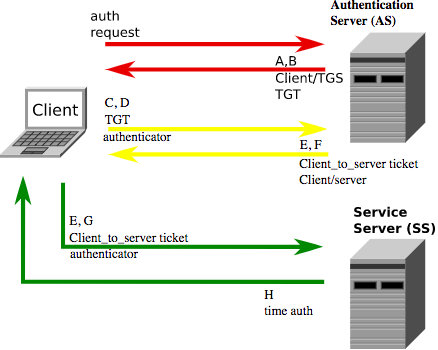
\includegraphics[width=0.5\textwidth]{Kerberos}
		\caption{Kerberos Authentication Procedure}
	\end{figure}
	
	Specifically, we need to deploy clusters secured by Kerberos, and then create a Kerberos principal with our username \& password in the Authentication Server(AS), and generate a encrypted keytab(key table) based on this principal. Since then, all authentications will be done based on this keytab, so that the password will not be exposed during transfer in networks. After that, we copy the encrypted keytab to our client machine and set its \href{https://en.wikipedia.org/wiki/File_system_permissions#Numeric_notation}{\textcolor{blue}{file permission}} as "-rwx------", which means read, write, \& execute only for owner. This ensures that other users are not allowed to access the keytab, so they have no chance to get authenticated as us. In the end, we execute the following command on the client machine to get authenticated and we can use all services like before, e.g. Livy, HDFS, Vora, etc.
	
	\noindent\textbf{kinit -k -t /etc/security/keytabs/livy.service.keytab username/realmname}
	
	After running this command, we are authenticated and have a ticket granting ticket(TGT), now we are allowed to send job submission requests. In addition, since we are authenticated, we cannot use Livy's impersonation feature anymore, so our security requirement is fulfilled.
	
	The command for secure job submission is a little bit different from the one in subsection 2.1:
	
	\noindent\textbf{curl -v --negotiate -u : \$LIVY\_URL/batches -X POST -H "Content-Type:application/json" -H "X-Requested-By: hdfs" --data '\{"file":"/tmp/spark-examples.jar","className":"org.apache.spark.examples.SparkPi","args":["10"]\}'}
	
	With the option "--negotiate -u :", curl is able to request client to server ticket from the AS, and then use this ticket to get Livy service from its Service Server(SS).
	
	Exactly same as the subsection 2.1, the job submission could be accepted and executed successfully. So it is proved that Livy could submit Spark jobs to a Kerberized cluster.
		
	\subsection{Prove that Livy could submit Vora jobs to a Kerberized cluster}
	
	At first, I thought that there is no difference between submitting a Vora job and a Spark job, but I was wrong - Kerberos protects not only the services Livy and Spark, but also Vora. Since Vora was still in development, there were 2 restrictions:
	
	\begin{enumerate}
		\item Almost all Kerberos configurations are hard-coded in the Vora and Spark config files, so changing Vora's Kerberos configurations is not supported;
		\item When Vora runs behind the Kerberos protection, it could be accessed only by the user vora, so in principle all the other users are not allowed to submit Vora jobs any more.
	\end{enumerate}
	
	This is a hard situation, that we cannot submit jobs as ourselves and we cannot change configurations to make it possible. In addition, as discussed in the chapter 2.3, theoretically once we are authenticated, we are not allowed to impersonate as another user such as the user vora.
	
	This difficulty made my work in a dilemma, I had proved everything but the most important part. After wasting almost 1 month for communicating with the security team in Turkey, and reading all kinds of documentations about Vora, Livy, and Kerberos, finally I found a very tricky solution - put users, which are allowed to use Vora, into Livy's superuser list. This makes it possible to let users get authenticated as themselves, and allow them to impersonate as the user vora so that they can submit Vora jobs as well.
	
	After submitting jobs and checking results as in the chapter 2.2, data is loaded into Vora, so it is proved that Livy could submit Vora jobs to a Kerberized cluster.\\
	
	Till now, the POC part is finally finished. The things I showed here is only a smart part of all I experienced, there were so many experiments and failures, but I can't write them all due to limited length. Anyway, I learned a lot during that time, the most important 2 things are:
	
	\begin{enumerate}
		\item Never simply believe in documentations, do experiments by yourself;
		\item Engineering is not perfectionism, tricky solutions are also solutions.
	\end{enumerate}
	
\newpage

\section{Source Code Implementation}
\setcounter{table}{0}
\setcounter{figure}{0}

After the POC of Livy was finished, I started to implement an Operator "Livy Spark Submit" in SAP Data Hub, specifically in the vFlow. With this operator, a pipeline could submit Spark/Vora jobs directly to any remote Hadoop cluster, no matter it's Kerberized or not. 

	\subsection{Requirements}
	In software engineering, code implementation is not the most difficult part, but understanding requirements. If the product cannot fulfill users' expectation, then it makes no sense no matter how many lines of code are written and how beautiful is the coding style. 
	
	However, requirements could change over time. Sometimes only after a requirement is implemented, people can find out it is useless or even wrong. Therefore, it is very important to keep communicating with people playing different roles. Although I am the only person writing code for this operator, there were always a weekly meeting, in which I, my tutor, the team leader, a security expert in Turkey and 3 technical consultants in the USA, shared the current development process, bugs, additional requirements and our opinions to the vision of this operator. Due to the length limit, I can't show all details we talked about. Let's simply see the final version of requirements for the operator "Livy Spark Submit":
	
	\begin{itemize}
		\item it works in SAP Data Hub Pipeline Modeler(vFlow);
		\item it could submit jobs to any remote cluster with Livy server;
		\item it could submit jobs to both simple and Kerberized clusters;
		\item it supports impersonation;
		\item it supports changing the name and configuration of jobs;
		\item it supports 2 error handling mode "default" and "pipeline". In the first mode, the pipeline fails when the operator fails. In the second mode, the operator's failure doesn't lead to pipelines failure, the operator outputs the error information via its output channel "outError";
		\item it supports 2 submission modes "jar" and "snippet". In the first mode it submits an job(application). In the second mode it maintains a session and sends several lines of spark code;
		\item for the "jar" mode, it specifies the path to the application jar, the class name and the arguments for execution;
		\item for the "snippet" mode, it specifies the code snippet and its language, and if the snippet is executed in the strict mode(the session stops when one line of code fails);
		\item it has 1 input channel. If no channel is set, it submits only once, when the whole pipeline is started. In the second way, it submits a job when an input signal arrives, no times limit;
		\item it has 2 output channels "outSuccess" and "outError" for outputting information when a job succeeds or fails.
	\end{itemize}
	
	\subsection{Implementation}
	\textbf{TODO: REST API}
	
	\textbf{TODO: JSON}
	
	
	\subsection{Refactoring}
	
	\subsection{New error handling mode}

\newpage

\section{Unit Tests \& Docker Based Integration Tests}
\setcounter{table}{0}
\setcounter{figure}{0}

Ambigitur quotiens, uter utro sit prior, aufert Pacuvius docti famam senis Accius alti, dicitur Afrani toga convenisse Menandro, Plautus. Hos ediscit et hos arto stipata theatro spectat Roma potens; habet hos nisi numeratque poetas ad ambigitur tempus Livi scriptoris ab aevo. Brevi vel toto est iunior anno. Interdum volgus rectum videt, est ubi peccat. Si veteres ita miratur laudatque poetas, ut nihil anteferat, nihil illis comparet, errat.  Si quaedam nimis antique, si peraque dure dicere credit eos, ignave multa fatetur, et sapit et mecum facit et Iova iudicat aequo. Non equidem insector delendave carmina Livi esse reor, memini quae plagosum mihi parvo Orbilium dictare; sed emendata videri pulchraque et exactis minimum distantia miror. Inter quae verbum emicuit si forte decorum, et si versus paulo concinnior unus et alter, venditque poema. Brevi vel toto est iunior anno. Utor permisso, caudaeque pilos ut equinae paulatim vello unum, demo etiam unum. Si meliora dies, ut vina, poemata reddit, scire velim, chartis perficit quotus pretium quotus arroget annus. Scriptor abhinc reddit misso annos centum qui decidit, inter perfectos veteresque referri debet an inter vilis atque perfectos novos? Excludat iurgia finis.
Est vetus atque probus, centum qui perficit annos. Quid, qui deperiitnihis perfectos uno mense vel? Iste quidem veteres inter ponetur honeste, qui vel mense brevi vel toto est iunior anno. Utor permisso, caudaeque nisi pilos ut equinae paulatim vello et virtutem, demo etiam unum, dum cadat elusus ratione ruentis acervi, qui redit in fastos et virtutem aestimat annis miraturque nihil nisi quod. Ennius et sapines et fortis et alter Homerus, ut critici dicunt, leviter curare videtur, quo promissa cadant et somnia Pythagorea.  Naevius in manibus non est et sanctum mentibus haeret paene recens?  Adeo sanctum est vetus omne poema. Ambigitur quotiens, uter utro sit prior, aufert Pacuvius docti famam senis:
\begin{itemize}\itemsep-\the\parsep
  \item Accius alti
  \item dicitur Afrani
  \item toga convenisse
  \item Menandro
  \item Plautus
\end{itemize}

\begin{center}
  \begin{longtable}[h!]
    {ll@{\kern5em}c@{\kern1.1em}c@{\kern1.1em}
    c@{\kern1.1em}c@{\kern1.1em}c@{\kern1.1em}c}
    \toprule
    \multirow{2}{*}{Name}&\multirow{2}{*}{Number}
    &\multicolumn{2}{c}{$d < 16$}&\multicolumn{2}{c}{$16 \leq d \leq 40$}&
    \multicolumn{2}{c}{$40 \leq 100$}\\\cmidrule(l{0.5em}r{0.5em}){3-8}
    & &$R_{p0,2}$ &$R_m$ &$R_{p0,2}$ &$R_m$ &$R_{p0,2}$ &$R_m$\\
    \cmidrule(l{0.5em}r{0.5em}){1-8}
    \endhead
    C 22 &1.0402 &$340$ &$500$ &$290$ &$470$ &$-$ &$-$\\
    C 22E &1.1151 &$340$ &$\cdots$ &$290$ &$\cdots$ &$-$ &$-$\\
    C 22R &1.1149 &$340$ &$650$ &$290$ &$620$ &$-$ &$-$\\
    \cmidrule(l{0.5em}r{0.5em}){1-8}
    C 25 &1.0406 &$370$ &$550$ &$320$ &$500$ &$-$ &$-$\\
    C 25E &1.1158 &$370$ &$\cdots$ &$320$ &$\cdots$ &$-$ &$-$\\
    C 25R &1.1163 &$370$ &$700$ &$320$ &$650$ &$-$ &$-$\\
    \cmidrule(l{0.5em}r{0.5em}){1-8}
    C 30 &1.0528 &$400$ &$600$ &$350$ &$550$ &$300$ &$500$\\
    \bottomrule
    \caption{$R_m$, $R_{eH}$ von Verg"utungsstahlen nach DIN EN 10 083-1/2: Mech.
      Eigenschaften der Stahle im Verg"uteten Zustand (+QT)}
  \end{longtable}
\end{center}

\newpage

\section{Conclusion}
\setcounter{table}{0}
\setcounter{figure}{0}

\newpage

\section*{Note of Thanks}\addcontentsline{toc}{section}{Note of Thanks}    \noindent
  Danke, danke, danke --- Danke vielmals --- Danke, sie k"onnen aufh"oren zu klatschen ---
  Wirklich --- Ach bitte setzen Sie sich doch --- Ja danke , danke\dots

\listoffigures\addcontentsline{toc}{section}{\listfigurename}
  
\end{document}
